\documentclass[11pt]{article}

\usepackage[margin=1in]{geometry}
\usepackage[T1]{fontenc}
\usepackage[utf8]{inputenc}
\usepackage{lmodern}
\usepackage{microtype}
\usepackage{amsmath,amssymb,amsthm,mathtools,bm}
\usepackage{booktabs,array,longtable,tabularx}
\usepackage{enumitem}
\usepackage{xcolor}
\usepackage{hyperref}
\usepackage[most]{tcolorbox}
\usepackage{tikz}
\usepackage{tikz-3dplot}
\usepackage{pgfplots}
\usepackage{caption}
\usepackage{float}
\usepackage{fancyhdr}
\usepackage{titlesec}

\pgfplotsset{compat=1.18}
\usetikzlibrary{arrows.meta,calc,positioning,patterns,decorations.pathreplacing,intersections,backgrounds,fit,matrix,3d}

\hypersetup{colorlinks=true,linkcolor=blue!55!black,urlcolor=blue!55!black,citecolor=blue!55!black}

\setlength{\headheight}{14pt}
\setlength{\parindent}{0pt}
\setlength{\parskip}{0.65em}
\setlist[itemize]{topsep=2pt,itemsep=2pt}
\setlist[enumerate]{topsep=2pt,itemsep=2pt}

\pagestyle{fancy}
\fancyhf{}
\lhead{Chapter 19. Vector Fields and Gradient Fields}
\rhead{\thepage}
\renewcommand{\headrulewidth}{0.4pt}

\titleformat{\section}{\large\bfseries\color{blue!55!black}}{\thesection}{0.6em}{}
\titleformat{\subsection}{\normalsize\bfseries\color{blue!45!black}}{\thesubsection}{0.6em}{}

\definecolor{chapterblue}{HTML}{1F5AA6}
\definecolor{chapterteal}{HTML}{168A8F}
\definecolor{chapterorange}{HTML}{D9822B}
\definecolor{chaptergreen}{HTML}{2D8A4E}
\definecolor{chapterpurple}{HTML}{6B4EAA}
\definecolor{chapterred}{HTML}{B23B3B}
\definecolor{softblue}{HTML}{EAF3FF}
\definecolor{softgreen}{HTML}{EAF8EF}
\definecolor{softorange}{HTML}{FFF4E6}
\definecolor{softpurple}{HTML}{F3EEFF}
\definecolor{softred}{HTML}{FFF0F0}
\definecolor{softgray}{HTML}{F6F7F9}
\definecolor{darkgray}{HTML}{30343B}

\newtcolorbox{chapteroverviewbox}{enhanced,breakable,colback=softblue,colframe=chapterblue,boxrule=0.8pt,arc=2mm,left=2mm,right=2mm,top=1mm,bottom=1mm}
\newtcolorbox{goalbox}{enhanced,breakable,colback=softgreen,colframe=chaptergreen,title=Learning goals,fonttitle=\bfseries,boxrule=0.8pt,arc=2mm}
\newtcolorbox{notebox}[1][]{enhanced,breakable,colback=softblue,colframe=chapterblue,title=#1,fonttitle=\bfseries,boxrule=0.7pt,arc=2mm}
\newtcolorbox{importantbox}[1][]{enhanced,breakable,colback=softred,colframe=chapterred,title=#1,fonttitle=\bfseries,boxrule=0.7pt,arc=2mm}
\newtcolorbox{tipbox}[1][]{enhanced,breakable,colback=softgreen,colframe=chaptergreen,title=#1,fonttitle=\bfseries,boxrule=0.7pt,arc=2mm}
\newtcolorbox{warningbox}[1][]{enhanced,breakable,colback=softorange,colframe=chapterorange,title=#1,fonttitle=\bfseries,boxrule=0.7pt,arc=2mm}
\newtcbtheorem[number within=section]{examplebox}{Example}{enhanced,breakable,colback=white,colframe=chapterblue,colbacktitle=chapterblue,fonttitle=\bfseries,boxrule=0.7pt,arc=1.5mm,left=2mm,right=2mm,top=1mm,bottom=1mm}{ex}

\newcommand{\R}{\mathbb R}
\newcommand{\grad}{\nabla}
\newcommand{\vect}[1]{\mathbf{#1}}
\newcommand{\norm}[1]{\left\lVert #1\right\rVert}
\newcommand{\dd}{\,d}
\newcommand{\ii}{\mathbf i}
\newcommand{\jj}{\mathbf j}
\newcommand{\kk}{\mathbf k}

\tikzset{
  vector/.style={-Latex,thick,chapterblue},
  fieldarrow/.style={-Latex,chapterblue!80!black,line width=0.6pt},
  fieldarrowred/.style={-Latex,chapterred!85!black,line width=0.6pt},
  fieldarrowteal/.style={-Latex,chapterteal!90!black,line width=0.6pt},
  contour/.style={chapterteal!70!black,thick},
  thincontour/.style={gray!60,thin},
  point/.style={circle,fill=chapterred,inner sep=1.6pt},
  boxnode/.style={draw=chapterblue,fill=softblue,rounded corners=2pt,align=center,inner sep=5pt,font=\small}
}

\begin{document}

\begin{center}
  {\LARGE\bfseries Chapter 19. Vector Fields and Gradient Fields\par}
  \vspace{0.35em}
  {\large From local arrows to global motion, force, and optimization\par}
\end{center}

\begin{chapteroverviewbox}
Scalar functions assign numbers to points. A temperature map assigns a temperature to each location, a density function assigns a density to each point in space, and a loss function assigns an error value to each parameter vector. Vector fields are different: they assign an arrow to each point.

This chapter begins the vector-calculus part of the book. We have already used vectors to describe geometry, curves, tangent directions, gradients, and optimization. Now vectors themselves become the output of a function. A vector field is the mathematical language of \emph{local direction}. It answers the question: if I stand at this point, which way does the field point, and how strongly?
\end{chapteroverviewbox}

\begin{goalbox}
After studying this chapter, you should be able to:
\begin{enumerate}
  \item define and visualize vector fields in $\R^2$, $\R^3$, and $\R^n$;
  \item distinguish scalar fields, vector fields, and vector-valued parameterized curves;
  \item sketch basic vector fields such as constant, radial, rotational, and gradient fields;
  \item compute gradient vector fields from scalar potential functions;
  \item recognize conservative vector fields and potential functions in simple cases;
  \item interpret vector fields as velocity fields, force fields, gradient flows, and optimization dynamics;
  \item use computation to visualize vector fields, gradient fields, and trajectories.
\end{enumerate}
\end{goalbox}

\begin{notebox}[Why this chapter matters]
Multiple integrals accumulate scalar quantities over regions. Vector calculus studies how vector quantities move through curves and surfaces. Before line integrals, flux, Green's theorem, Stokes' theorem, or the divergence theorem, we need a precise understanding of vector fields.
\end{notebox}

\section{Scalar fields versus vector fields}

A \textbf{scalar field} assigns one number to each point. For example,
\[
f(x,y)=x^2+y^2
\]
assigns a scalar height, temperature, loss, or density value to each point $(x,y)$.

A \textbf{vector field} assigns a vector to each point. For example,
\[
F(x,y)=\langle -y,x\rangle
\]
assigns the vector $\langle -y,x\rangle$ to the point $(x,y)$. At $(1,0)$, it gives $\langle 0,1\rangle$. At $(0,1)$, it gives $\langle -1,0\rangle$.

\begin{importantbox}[Three different objects]
Do not confuse these objects:
\begin{itemize}
  \item a scalar field has the form $f:\R^n\to\R$;
  \item a vector field has the form $F:\R^n\to\R^n$;
  \item a parameterized curve has the form $r:I\to\R^n$.
\end{itemize}
A curve uses one parameter to trace points. A vector field places an arrow at many points.
\end{importantbox}

\begin{figure}[H]
\centering
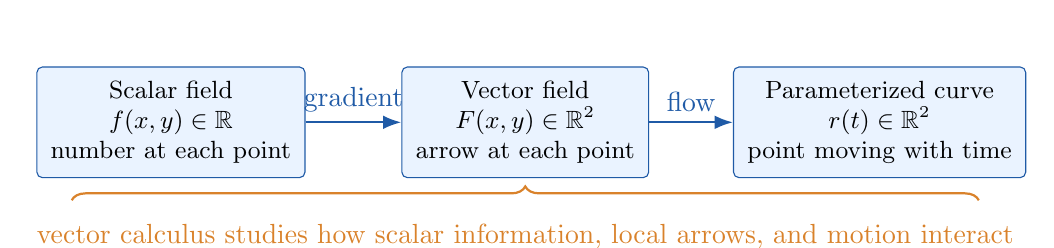
\begin{tikzpicture}[scale=0.9]
\node[boxnode] (scalar) at (0,0) {Scalar field\\$f(x,y)\in\R$\\number at each point};
\node[boxnode] (vector) at (5,0) {Vector field\\$F(x,y)\in\R^2$\\arrow at each point};
\node[boxnode] (curve) at (10,0) {Parameterized curve\\$r(t)\in\R^2$\\point moving with time};
\draw[vector] (scalar) -- node[above]{gradient} (vector);
\draw[vector] (vector) -- node[above]{flow} (curve);
\draw[chapterorange,thick,decorate,decoration={brace,amplitude=5pt}] (-1.4,-1.1) -- (11.4,-1.1) node[midway,below=5pt,align=center]{vector calculus studies how scalar information, local arrows, and motion interact};
\end{tikzpicture}
\caption{Three related but distinct objects. A gradient transforms a scalar field into a vector field, and a vector field can generate motion.}
\end{figure}

\section{Vector fields in the plane}

A vector field on a region $D\subseteq\R^2$ is a function
\[
F(x,y)=\langle P(x,y),Q(x,y)\rangle
\]
that assigns to each point $(x,y)\in D$ a two-dimensional vector. Here $P$ is the horizontal component and $Q$ is the vertical component. In unit-vector notation,
\[
F(x,y)=P(x,y)\ii+Q(x,y)\jj.
\]

\begin{examplebox}{Constant, downward, and rotational fields}{basicfields}
The field $F(x,y)=\langle 1,0\rangle$ places the same right-pointing vector at every point. The field $G(x,y)=\langle 0,-1\rangle$ places the same downward vector at every point. The field
\[
R(x,y)=\langle -y,x\rangle
\]
is tangent to circles centered at the origin because
\[
\langle -y,x\rangle\cdot \langle x,y\rangle=-xy+xy=0.
\]
This field rotates counterclockwise around the origin.
\end{examplebox}

\begin{figure}[H]
\centering
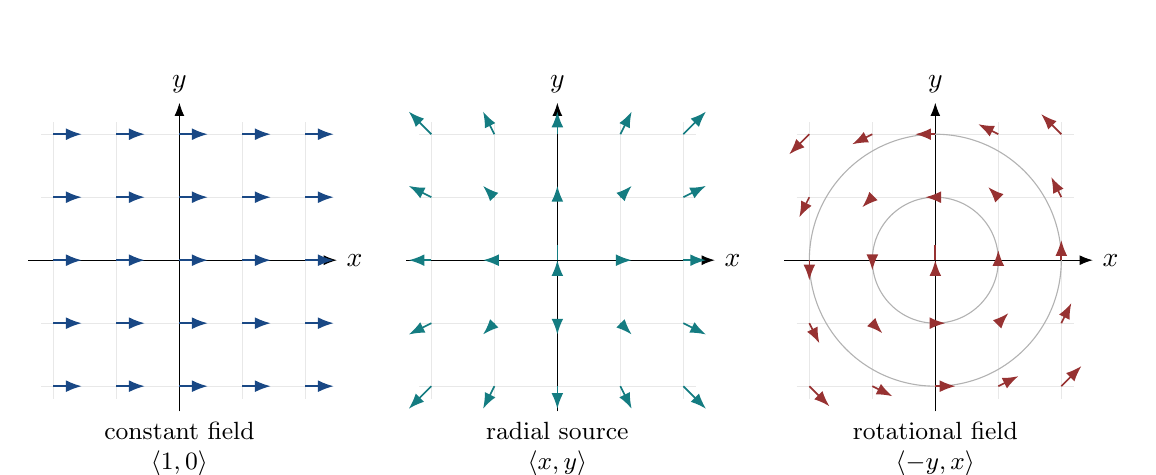
\begin{tikzpicture}[scale=0.8]
% panel 1 constant
\begin{scope}[shift={(0,0)}]
\draw[step=1,gray!18] (-2.2,-2.2) grid (2.2,2.2);
\draw[-Latex] (-2.4,0)--(2.5,0) node[right]{$x$};
\draw[-Latex] (0,-2.4)--(0,2.5) node[above]{$y$};
\foreach \x in {-2,-1,0,1,2}{\foreach \y in {-2,-1,0,1,2}{\draw[fieldarrow] (\x,\y)--++(0.45,0);}}
\node[align=center,font=\small] at (0,-3.0) {constant field\\$\langle 1,0\rangle$};
\end{scope}
% panel 2 radial
\begin{scope}[shift={(6,0)}]
\draw[step=1,gray!18] (-2.2,-2.2) grid (2.2,2.2);
\draw[-Latex] (-2.4,0)--(2.5,0) node[right]{$x$};
\draw[-Latex] (0,-2.4)--(0,2.5) node[above]{$y$};
\foreach \x in {-2,-1,0,1,2}{\foreach \y in {-2,-1,0,1,2}{\pgfmathsetmacro{\u}{0.18*\x}\pgfmathsetmacro{\v}{0.18*\y}\draw[fieldarrowteal] (\x,\y)--++(\u,\v);}}
\node[align=center,font=\small] at (0,-3.0) {radial source\\$\langle x,y\rangle$};
\end{scope}
% panel 3 rotational
\begin{scope}[shift={(12,0)}]
\draw[step=1,gray!18] (-2.2,-2.2) grid (2.2,2.2);
\draw[-Latex] (-2.4,0)--(2.5,0) node[right]{$x$};
\draw[-Latex] (0,-2.4)--(0,2.5) node[above]{$y$};
\draw[thincontour] (0,0) circle (1);
\draw[thincontour] (0,0) circle (2);
\foreach \x in {-2,-1,0,1,2}{\foreach \y in {-2,-1,0,1,2}{\pgfmathsetmacro{\u}{-0.16*\y}\pgfmathsetmacro{\v}{0.16*\x}\draw[fieldarrowred] (\x,\y)--++(\u,\v);}}
\node[align=center,font=\small] at (0,-3.0) {rotational field\\$\langle -y,x\rangle$};
\end{scope}
\end{tikzpicture}
\caption{Constant, radial, and rotational vector fields in the plane. The same grid of points can carry very different local directions.}
\end{figure}

\section{Vector fields in space and high dimensions}

A vector field in three-dimensional space has the form
\[
F(x,y,z)=\langle P(x,y,z),Q(x,y,z),R(x,y,z)\rangle.
\]
For example, $F(x,y,z)=\langle x,y,z\rangle$ points radially outward from the origin, while $G(x,y,z)=\langle -y,x,0\rangle$ rotates around the $z$-axis.

More generally, in $\R^n$ a vector field has the form
\[
F(x_1,\ldots,x_n)=\langle F_1(x),F_2(x),\ldots,F_n(x)\rangle.
\]
High-dimensional vector fields appear in optimization and machine learning, where a point represents a parameter vector and the arrow represents a parameter update direction.

\begin{figure}[H]
\centering
\tdplotsetmaincoords{65}{115}
\begin{tikzpicture}[tdplot_main_coords,scale=1.05]
\draw[-Latex] (0,0,0)--(3,0,0) node[below left]{$x$};
\draw[-Latex] (0,0,0)--(0,3,0) node[right]{$y$};
\draw[-Latex] (0,0,0)--(0,0,3) node[above]{$z$};
\foreach \x/\y/\z in {0.8/0.5/0.5,1.6/0.5/0.8,0.5/1.6/0.9,1.7/1.6/1.2,0.7/0.8/2.0,1.8/0.9/2.2}{
  \pgfmathsetmacro{\u}{0.22*\x}
  \pgfmathsetmacro{\v}{0.22*\y}
  \pgfmathsetmacro{\w}{0.22*\z}
  \fill[chapterred] (\x,\y,\z) circle (1.1pt);
  \draw[-Latex,chapterblue,thick] (\x,\y,\z)--({\x+\u},{\y+\v},{\z+\w});
}
\draw[chapterteal!50,fill=chapterteal!8,opacity=0.6] (0,0,0)--(2.4,0,0)--(2.4,2.4,0)--(0,2.4,0)--cycle;
\node[align=center] at (2.5,2.1,2.6) {$F(x,y,z)=\langle x,y,z\rangle$\\radial field in space};
\end{tikzpicture}
\caption{A vector field in $\R^3$ assigns a three-dimensional arrow to each point in space.}
\end{figure}

\section{Gradient fields}

If $f$ is a scalar field, then its gradient is a vector field. In the plane,
\[
\grad f(x,y)=\langle f_x(x,y),f_y(x,y)\rangle.
\]
In space,
\[
\grad f(x,y,z)=\langle f_x(x,y,z),f_y(x,y,z),f_z(x,y,z)\rangle.
\]
A vector field $F$ is called a \textbf{gradient field} if there exists a scalar function $f$ such that
\[
F=\grad f.
\]
The function $f$ is called a \textbf{potential function} for $F$.

\begin{tipbox}[Geometry of a gradient field]
A gradient vector field is perpendicular to level curves or level surfaces of its potential. The arrows point uphill; the negative gradient points downhill.
\end{tipbox}

\begin{examplebox}{A quadratic potential}{quadraticpotential}
Let
\[
f(x,y)=\frac12 x^2+y^2.
\]
Then
\[
\grad f(x,y)=\langle x,2y\rangle.
\]
The level curves of $f$ are ellipses. The gradient vectors are perpendicular to those ellipses and point outward toward larger values of $f$.
\end{examplebox}

\begin{figure}[H]
\centering
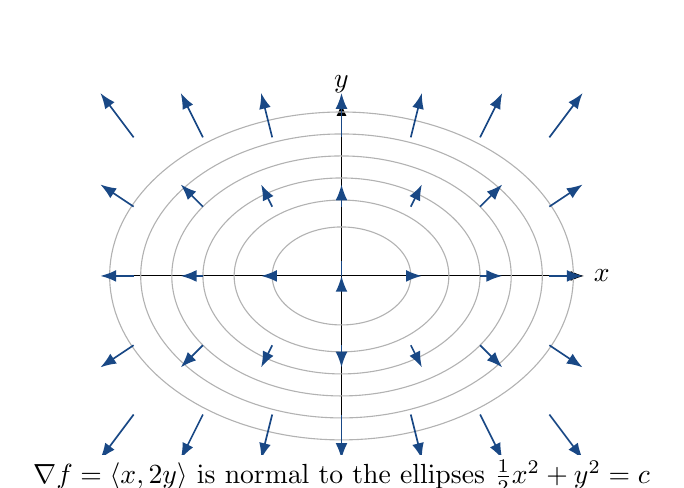
\begin{tikzpicture}[scale=0.88]
\draw[-Latex] (-3.4,0)--(3.5,0) node[right]{$x$};
\draw[-Latex] (0,-2.4)--(0,2.5) node[above]{$y$};
\foreach \c in {0.5,1.2,2.0,3.0,4.2,5.6}{
  \pgfmathsetmacro{\rx}{sqrt(2*\c)}
  \pgfmathsetmacro{\ry}{sqrt(\c)}
  \draw[thincontour] plot[domain=0:360,samples=160] ({\rx*cos(\x)},{\ry*sin(\x)});
}
\foreach \x in {-3,-2,-1,0,1,2,3}{\foreach \y in {-2,-1,0,1,2}{
  \pgfmathsetmacro{\u}{0.16*\x}
  \pgfmathsetmacro{\v}{0.32*\y}
  \draw[fieldarrow] (\x,\y)--++(\u,\v);
}}
\node[align=center,fill=white,inner sep=2pt] at (0,-2.9) {$\grad f=\langle x,2y\rangle$ is normal to the ellipses $\frac12x^2+y^2=c$};
\end{tikzpicture}
\caption{Gradient field of a quadratic potential. The arrows are perpendicular to the level curves.}
\end{figure}

\begin{examplebox}{Computing gradient fields}{computegrad}
For
\[
f(x,y)=\sin(xy)+e^y,
\]
we have
\[
f_x(x,y)=y\cos(xy),\qquad f_y(x,y)=x\cos(xy)+e^y.
\]
Therefore
\[
\grad f(x,y)=\langle y\cos(xy),x\cos(xy)+e^y\rangle.
\]
For a three-dimensional example, if $f(x,y,z)=xyz$, then
\[
\grad f(x,y,z)=\langle yz,xz,xy\rangle,
\qquad
\grad f(1,2,3)=\langle 6,3,2\rangle.
\]
\end{examplebox}

\section{Gradient fields and optimization}

In optimization, the scalar function is often a loss function $L(\theta)$, where $\theta$ is a vector of parameters. The gradient field
\[
\grad L(\theta)
\]
points in the direction of fastest increase of the loss. Gradient descent follows the negative gradient:
\[
\theta_{k+1}=\theta_k-\alpha\grad L(\theta_k).
\]
This is also a discrete approximation to a continuous vector field flow:
\[
\frac{d\theta}{dt}=-\grad L(\theta).
\]
Thus optimization can be viewed as motion in a vector field.

\begin{figure}[H]
\centering
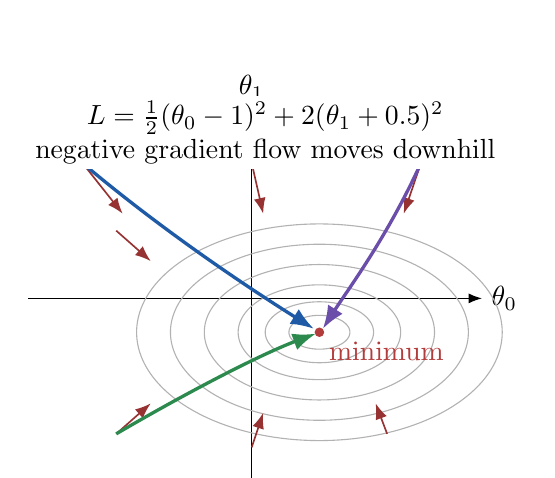
\begin{tikzpicture}[scale=0.86]
\draw[-Latex] (-3.3,0)--(3.4,0) node[right]{$\theta_0$};
\draw[-Latex] (0,-2.8)--(0,2.8) node[above]{$\theta_1$};
\coordinate (m) at (1,-0.5);
\foreach \a/\b in {0.45/0.25,0.8/0.45,1.2/0.7,1.7/1.0,2.2/1.3,2.7/1.6}{
  \draw[thincontour] plot[domain=0:360,samples=160] ({1+\a*cos(\x)},{-0.5+\b*sin(\x)});
}
\fill[chapterred] (m) circle (2pt) node[below right] {minimum};
\foreach \x/\y in {-2.5/2.0,-2/1,0/2,2.5/2,2/-2,-2/-2,0/-2.2}{
  \pgfmathsetmacro{\u}{-0.17*(\x-1)}
  \pgfmathsetmacro{\v}{-0.30*(\y+0.5)}
  \draw[fieldarrowred] (\x,\y)--++(\u,\v);
}
\draw[chapterblue,very thick,-Latex] (-2.5,2.0) .. controls (-1.2,0.9) and (0.2,0.0) .. (0.92,-0.45);
\draw[chapterpurple,very thick,-Latex] (2.5,2.0) .. controls (2.0,0.9) and (1.4,0.1) .. (1.05,-0.45);
\draw[chaptergreen,very thick,-Latex] (-2,-2) .. controls (-0.8,-1.3) and (0.2,-0.8) .. (0.95,-0.52);
\node[align=center,fill=white,inner sep=2pt] at (0.2,2.45) {$L=\frac12(\theta_0-1)^2+2(\theta_1+0.5)^2$\\negative gradient flow moves downhill};
\end{tikzpicture}
\caption{Gradient descent follows the negative gradient field toward smaller values of the loss.}
\end{figure}

\section{Conservative vector fields}

A vector field $F$ is \textbf{conservative} if it is the gradient of some potential function:
\[
F=\grad f.
\]
For example,
\[
F(x,y)=\langle 2x,2y\rangle
\]
is conservative because $F=\grad(x^2+y^2)$. The potential function is not unique: adding a constant does not change the gradient. Thus $x^2+y^2+C$ has the same gradient field for every constant $C$.

\subsection*{How to find a potential function}
Suppose
\[
F(x,y)=\langle P(x,y),Q(x,y)\rangle.
\]
To find a potential function $f$, we want
\[
f_x=P,\qquad f_y=Q.
\]
A practical method is:
\begin{enumerate}
  \item integrate $P$ with respect to $x$;
  \item include an unknown function of $y$;
  \item differentiate with respect to $y$ and compare with $Q$.
\end{enumerate}

\begin{examplebox}{Finding a potential}{potentialfind}
Let
\[
F(x,y)=\langle y^2-3x^2,2xy\rangle.
\]
We seek $f$ such that $f_x=y^2-3x^2$. Integrating with respect to $x$ gives
\[
f(x,y)=xy^2-x^3+g(y),
\]
where $g(y)$ is unknown. Differentiate with respect to $y$:
\[
f_y=2xy+g'(y).
\]
Since we need $f_y=2xy$, we get $g'(y)=0$. Therefore $g$ is constant, and one potential function is
\[
f(x,y)=xy^2-x^3.
\]
\end{examplebox}

\section{A quick test in the plane}

For many fields on simple domains, a useful test is based on mixed partial derivatives. If
\[
F(x,y)=\langle P(x,y),Q(x,y)\rangle
\]
is a gradient field, then $P=f_x$ and $Q=f_y$. Therefore
\[
P_y=f_{xy},\qquad Q_x=f_{yx}.
\]
When the relevant second partial derivatives are continuous, equality of mixed partials gives
\[
P_y=Q_x.
\]
This condition is necessary for being a gradient field, and on many simple regions it is also sufficient. A complete treatment comes later when we study line integrals and Green's theorem.

\begin{examplebox}{Radial fields versus rotational fields}{gradvsrot}
For $F(x,y)=\langle -y,x\rangle$, we have $P_y=-1$ and $Q_x=1$. Since $P_y\ne Q_x$, this field is not a gradient field on the plane. By contrast, for $F(x,y)=\langle x,y\rangle$, we have $P_y=0$ and $Q_x=0$, and indeed
\[
F=\grad\left(\frac12x^2+\frac12y^2\right).
\]
\end{examplebox}

\begin{figure}[H]
\centering
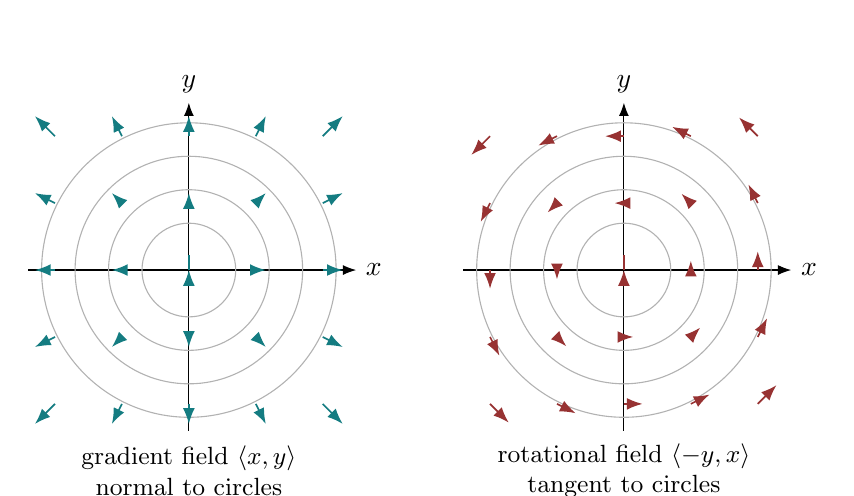
\begin{tikzpicture}[scale=0.85]
\begin{scope}[shift={(0,0)}]
\draw[-Latex] (-2.4,0)--(2.5,0) node[right]{$x$};
\draw[-Latex] (0,-2.4)--(0,2.5) node[above]{$y$};
\foreach \r in {0.7,1.2,1.7,2.2}{\draw[thincontour] (0,0) circle (\r);}
\foreach \x in {-2,-1,0,1,2}{\foreach \y in {-2,-1,0,1,2}{\pgfmathsetmacro{\u}{0.15*\x}\pgfmathsetmacro{\v}{0.15*\y}\draw[fieldarrowteal] (\x,\y)--++(\u,\v);}}
\node[align=center,font=\small] at (0,-3) {gradient field $\langle x,y\rangle$\\normal to circles};
\end{scope}
\begin{scope}[shift={(6.5,0)}]
\draw[-Latex] (-2.4,0)--(2.5,0) node[right]{$x$};
\draw[-Latex] (0,-2.4)--(0,2.5) node[above]{$y$};
\foreach \r in {0.7,1.2,1.7,2.2}{\draw[thincontour] (0,0) circle (\r);}
\foreach \x in {-2,-1,0,1,2}{\foreach \y in {-2,-1,0,1,2}{\pgfmathsetmacro{\u}{-0.14*\y}\pgfmathsetmacro{\v}{0.14*\x}\draw[fieldarrowred] (\x,\y)--++(\u,\v);}}
\node[align=center,font=\small] at (0,-3) {rotational field $\langle -y,x\rangle$\\tangent to circles};
\end{scope}
\end{tikzpicture}
\caption{A gradient field has arrows normal to level curves, while a rotational field circulates around them.}
\end{figure}

\section{Vector fields as differential equations}

A vector field can define motion. If
\[
F(x,y)=\langle P(x,y),Q(x,y)\rangle,
\]
then a trajectory following the field satisfies
\[
\frac{dx}{dt}=P(x,y),\qquad \frac{dy}{dt}=Q(x,y).
\]
In vector form,
\[
\frac{dr}{dt}=F(r(t)).
\]
The vector field tells the particle's velocity at each point. The trajectory is a curve whose tangent vector agrees with the field.

\begin{examplebox}{Rotation around the origin}{rotationode}
For $F(x,y)=\langle -y,x\rangle$, the motion equations are
\[
\frac{dx}{dt}=-y,\qquad \frac{dy}{dt}=x.
\]
The solutions move around circles centered at the origin. The vector field is tangent to those circles.
\end{examplebox}

\begin{figure}[H]
\centering
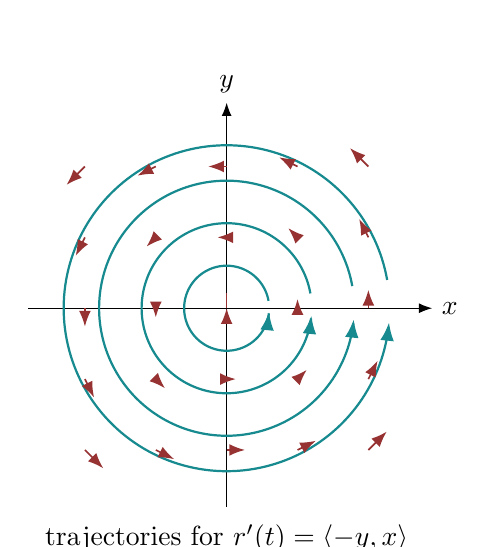
\begin{tikzpicture}[scale=0.9]
\draw[-Latex] (-2.8,0)--(2.9,0) node[right]{$x$};
\draw[-Latex] (0,-2.8)--(0,2.9) node[above]{$y$};
\foreach \r in {0.6,1.2,1.8,2.3}{
  \draw[chapterteal,thick,-Latex] plot[domain=10:355,samples=180] ({\r*cos(\x)},{\r*sin(\x)});
}
\foreach \x in {-2,-1,0,1,2}{\foreach \y in {-2,-1,0,1,2}{\pgfmathsetmacro{\u}{-0.13*\y}\pgfmathsetmacro{\v}{0.13*\x}\draw[fieldarrowred] (\x,\y)--++(\u,\v);}}
\node[align=center,fill=white,inner sep=2pt] at (0,-3.25) {trajectories for $r'(t)=\langle -y,x\rangle$};
\end{tikzpicture}
\caption{Trajectories following the rotational field move around circles.}
\end{figure}

\section{Sources, sinks, and radial flow}

The radial field $F(x,y)=\langle x,y\rangle$ points away from the origin. It behaves like a \textbf{source}: trajectories move outward. The negative radial field $F(x,y)=\langle -x,-y\rangle$ points toward the origin. It behaves like a \textbf{sink}: trajectories move inward.

In optimization, a sink often represents a local minimum of a loss function. If $L(x,y)=\frac12(x^2+y^2)$, then
\[
-\grad L(x,y)=\langle -x,-y\rangle.
\]
So the negative gradient flow moves toward the minimizer at the origin.

\begin{figure}[H]
\centering
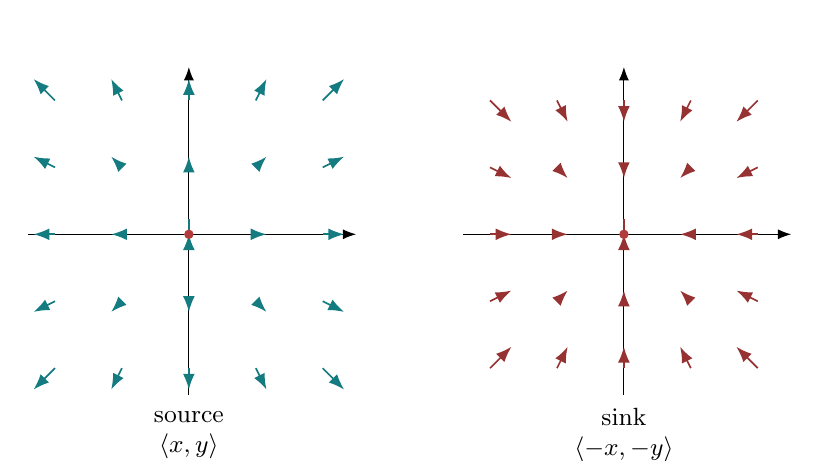
\begin{tikzpicture}[scale=0.85]
\begin{scope}[shift={(0,0)}]
\draw[-Latex] (-2.4,0)--(2.5,0);
\draw[-Latex] (0,-2.4)--(0,2.5);
\foreach \x in {-2,-1,0,1,2}{\foreach \y in {-2,-1,0,1,2}{\pgfmathsetmacro{\u}{0.16*\x}\pgfmathsetmacro{\v}{0.16*\y}\draw[fieldarrowteal] (\x,\y)--++(\u,\v);}}
\fill[chapterred] (0,0) circle (2pt);
\node[align=center,font=\small] at (0,-3) {source\\$\langle x,y\rangle$};
\end{scope}
\begin{scope}[shift={(6.5,0)}]
\draw[-Latex] (-2.4,0)--(2.5,0);
\draw[-Latex] (0,-2.4)--(0,2.5);
\foreach \x in {-2,-1,0,1,2}{\foreach \y in {-2,-1,0,1,2}{\pgfmathsetmacro{\u}{-0.16*\x}\pgfmathsetmacro{\v}{-0.16*\y}\draw[fieldarrowred] (\x,\y)--++(\u,\v);}}
\fill[chapterred] (0,0) circle (2pt);
\node[align=center,font=\small] at (0,-3) {sink\\$\langle -x,-y\rangle$};
\end{scope}
\end{tikzpicture}
\caption{Source and sink vector fields. The source points outward; the sink points inward.}
\end{figure}

\section{Vector fields in probability and statistics}

Vector fields also appear in probability and statistics. For a positive density $p(x)$ on $\R^n$, the vector field
\[
s(x)=\grad \log p(x)
\]
is called the \textbf{score field}. It points toward directions where the log-density increases.

For the standard Gaussian density in two dimensions,
\[
p(x,y)=\frac{1}{2\pi}e^{-(x^2+y^2)/2},
\]
we have
\[
\log p(x,y)=C-\frac12(x^2+y^2),
\]
so
\[
\grad\log p(x,y)=\langle -x,-y\rangle.
\]
Thus the score field points toward the high-density region at the origin.

\begin{figure}[H]
\centering
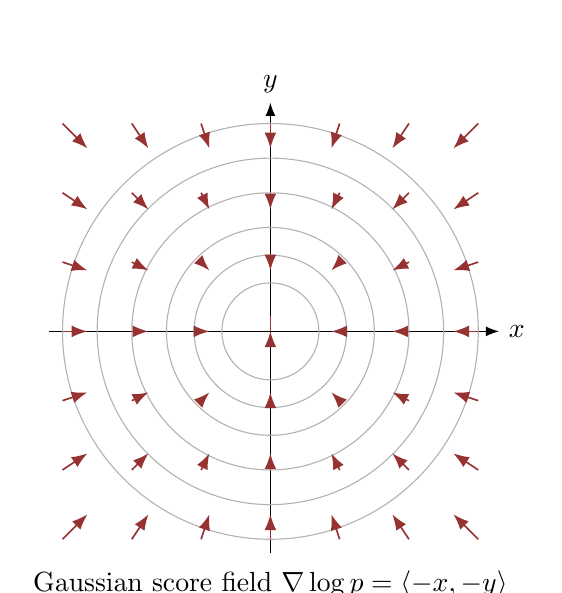
\begin{tikzpicture}[scale=0.88]
\draw[-Latex] (-3.2,0)--(3.3,0) node[right]{$x$};
\draw[-Latex] (0,-3.2)--(0,3.3) node[above]{$y$};
\foreach \r in {0.7,1.1,1.5,2.0,2.5,3.0}{\draw[thincontour] (0,0) circle (\r);}
\foreach \x in {-3,-2,-1,0,1,2,3}{\foreach \y in {-3,-2,-1,0,1,2,3}{\pgfmathsetmacro{\u}{-0.12*\x}\pgfmathsetmacro{\v}{-0.12*\y}\draw[fieldarrowred] (\x,\y)--++(\u,\v);}}
\node[fill=white,inner sep=2pt] at (0,-3.65) {Gaussian score field $\grad\log p=\langle -x,-y\rangle$};
\end{tikzpicture}
\caption{The score field of a standard bivariate Gaussian points toward the center of highest density.}
\end{figure}

This is one reason vector fields are increasingly important in modern statistics and machine learning: they describe how probability mass, particles, parameters, and samples move.

\section{A field guide to common vector fields}

\begin{center}
\begin{tabularx}{\textwidth}{@{}>{\bfseries}l>{\centering\arraybackslash}X X@{}}
\toprule
Field & Formula & Main behavior \\
\midrule
Constant field & $\langle a,b\rangle$ & uniform direction and magnitude \\
Radial source & $\langle x,y\rangle$ & points away from origin \\
Radial sink & $\langle -x,-y\rangle$ & points toward origin \\
Rotational field & $\langle -y,x\rangle$ & circulates counterclockwise \\
Gradient field & $\grad f$ & points toward fastest increase of $f$ \\
Negative gradient field & $-\grad f$ & points toward fastest decrease of $f$ \\
Singular radial field & $\langle x,y\rangle/(x^2+y^2)$ & radial with singularity at origin \\
\bottomrule
\end{tabularx}
\end{center}

\section{Worked examples}

\begin{examplebox}{Classify and interpret a field}{classifyfield}
Consider
\[
F(x,y)=\langle 2x,8y\rangle.
\]
We look for $f$ such that $f_x=2x$ and $f_y=8y$. Integrating $f_x=2x$ with respect to $x$ gives
\[
f(x,y)=x^2+g(y).
\]
Then $f_y=g'(y)$, so we need $g'(y)=8y$. Hence $g(y)=4y^2+C$, and one potential is
\[
f(x,y)=x^2+4y^2.
\]
The level curves $x^2+4y^2=c$ are ellipses. The vector field points outward and is perpendicular to these ellipses. The negative field $-F(x,y)=\langle -2x,-8y\rangle$ would drive points toward the minimum at $(0,0)$.
\end{examplebox}

\begin{examplebox}{Testing conservative behavior}{conservativecheck}
Let $F(x,y)=\langle y,x+y\rangle$. Here $P_y=1$ and $Q_x=1$, so the mixed-partial test passes. Find a potential by solving $f_x=y$. Integrating gives
\[
f(x,y)=xy+g(y).
\]
Then $f_y=x+g'(y)$. Since $f_y=x+y$, we need $g'(y)=y$, so $g(y)=\frac12y^2$. Hence
\[
f(x,y)=xy+\frac12y^2.
\]
For $H(x,y)=\langle -y,x\rangle$, however, $P_y=-1$ and $Q_x=1$, so the field cannot be a gradient field on the plane.
\end{examplebox}

\begin{notebox}[What comes next]
In the next chapter, we integrate functions along curves. For a scalar field, a line integral measures accumulated density along a curve. For a vector field, a line integral measures accumulated tangential work. Conservative fields will become powerful because their work integrals depend only on endpoints.
\end{notebox}

\section{Python lab: building and visualizing vector fields}

The Python lab for this chapter focuses on:
\begin{itemize}
  \item comparing scalar fields, vector fields, and trajectories;
  \item plotting constant, radial, rotational, and singular vector fields;
  \item computing gradient vector fields from potential functions;
  \item visualizing negative gradient flow and gradient descent paths;
  \item exploring score fields from probability models.
\end{itemize}

A reusable helper has the form
\[
(P,Q)\mapsto \text{a quiver plot of }F(x,y)=\langle P(x,y),Q(x,y)\rangle.
\]
For example, plotting $F(x,y)=\langle x-y,x+y\rangle$ reveals a combination of stretching and rotation.

\section{Chapter summary}

A vector field assigns an arrow to each point. In the plane it has the form
\[
F(x,y)=\langle P(x,y),Q(x,y)\rangle,
\]
and in space it has the form
\[
F(x,y,z)=\langle P(x,y,z),Q(x,y,z),R(x,y,z)\rangle.
\]
The most important special case is a gradient field:
\[
F=\grad f.
\]
Gradient fields arise from scalar potentials. They are perpendicular to level curves and level surfaces, and they point in the direction of fastest increase. Negative gradient fields describe descent, optimization, stable motion toward minima, and score-based movement toward high-density regions.

Vector fields prepare us for line integrals, work, circulation, flux, curl, divergence, Green's theorem, Stokes' theorem, and the divergence theorem.

\section{Exercises}

\subsection*{Conceptual exercises}
\begin{enumerate}
  \item Explain the difference between a scalar field and a vector field.
  \item Give one physical example and one data-science example of a vector field.
  \item Why is $F(x,y)=\langle -y,x\rangle$ tangent to circles centered at the origin?
  \item Explain why a gradient field is perpendicular to level curves of its potential.
  \item What does it mean for a vector field to have a singularity?
  \item In optimization, why do we usually follow $-\grad L$ instead of $\grad L$?
\end{enumerate}

\subsection*{Computational exercises}
\begin{enumerate}
  \item Sketch $F(x,y)=\langle x,0\rangle$ by hand and describe its behavior.
  \item Sketch $F(x,y)=\langle 0,y\rangle$ by hand and describe its behavior.
  \item Sketch $F(x,y)=\langle y,x\rangle$. Is it radial, rotational, or neither?
  \item Compute the gradient field of $f(x,y)=x^2+xy+y^2$.
  \item Compute the gradient field of $f(x,y,z)=x^2y+yz^2$.
  \item Find a potential function for $F(x,y)=\langle 3x^2+y,x+2y\rangle$.
  \item Decide whether $F(x,y)=\langle y^2,2xy\rangle$ is a gradient field. If so, find a potential.
  \item Decide whether $F(x,y)=\langle x-y,x+y\rangle$ can be a gradient field on the plane.
  \item Let $F(x,y)=\langle -x,-y\rangle$. Solve $r'(t)=F(r(t))$ with $r(0)=(a,b)$.
  \item Let $F(x,y)=\langle -y,x\rangle$. Show that $x(t)^2+y(t)^2$ is constant along trajectories.
\end{enumerate}

\subsection*{Applied exercises}
\begin{enumerate}
  \item Suppose $L(\theta_0,\theta_1)=(\theta_0-2)^2+3(\theta_1+1)^2$. Compute the negative gradient field and identify the minimizer.
  \item For the density $p(x,y)=Ce^{-(x^2+4y^2)/2}$, compute the score field $\grad\log p$.
  \item A velocity field is $F(x,y)=\langle 1+y,1-x\rangle$. Compute the velocity at $(0,0)$, $(1,0)$, and $(0,1)$.
  \item A force field is $F(x,y,z)=\langle x,y,z\rangle$. What is the magnitude of the force at $(1,2,2)$?
  \item Plot $F(x,y)=\langle \sin y,\cos x\rangle$ and describe its visible behavior.
  \item Plot the negative gradient field of $f(x,y)=x^4+y^4-4xy$. Locate possible stable points visually.
\end{enumerate}

\subsection*{Challenge exercises}
\begin{enumerate}
  \item Let $F=\langle P,Q\rangle$ be a gradient field with potential $f$. Explain why the vector field is zero at every critical point of $f$.
  \item Find all points where $F(x,y)=\langle x^2-y^2,2xy\rangle$ is zero.
  \item Let $F(x,y)=\langle ax+by,cx+dy\rangle$. Find a condition on $a,b,c,d$ that is necessary for $F$ to be a gradient field.
  \item Suppose $F=\grad f$ and $f$ has a strict local minimum at $p$. What does the negative gradient field usually do near $p$?
  \item Consider $F(x,y)=\langle -y/(x^2+y^2),x/(x^2+y^2)\rangle$ on $\R^2\setminus\{0\}$. Check the mixed-partial condition and describe what the field looks like.
\end{enumerate}

\section{Chapter project: vector fields behind gradient descent}

Choose a differentiable loss function $L(\theta_0,\theta_1)$ with at least one local minimum. Analyze the vector field
\[
F(\theta_0,\theta_1)=-\grad L(\theta_0,\theta_1).
\]
Your report should include:
\begin{enumerate}
  \item the formula for $L$;
  \item the formula for $\grad L$;
  \item a contour plot of $L$;
  \item a quiver plot of $-\grad L$;
  \item several gradient descent paths from different starting points;
  \item a short explanation of what the field reveals about the geometry of the loss surface.
\end{enumerate}
This project connects multivariable calculus directly to optimization in statistics, machine learning, and artificial intelligence.

\end{document}
